\section{Datenübertragung}
\label{sec:Daten}
Im Folgenden wird das Konzept beschrieben, um Daten des VARAN-Buses optisch und bidirektional auf den Drehteller zu übertragen und somit ein Datenkabel hinfällig wird. Ausserdem wird eine Sende- und Empfängerschaltung entworfen, um eine unidirektionale Übertragung mit zwei Pegeln zu testen und wichtige Erkenntnisse für die Fortsetzung der Arbeit zu sammeln.  
\subsection{Konzept}
In Abbildung \ref{fig:Konzept_Daten} wird grob das Konzept zur optischen Datenübertragung gezeigt.

\begin{figure}[h]
	\centering
	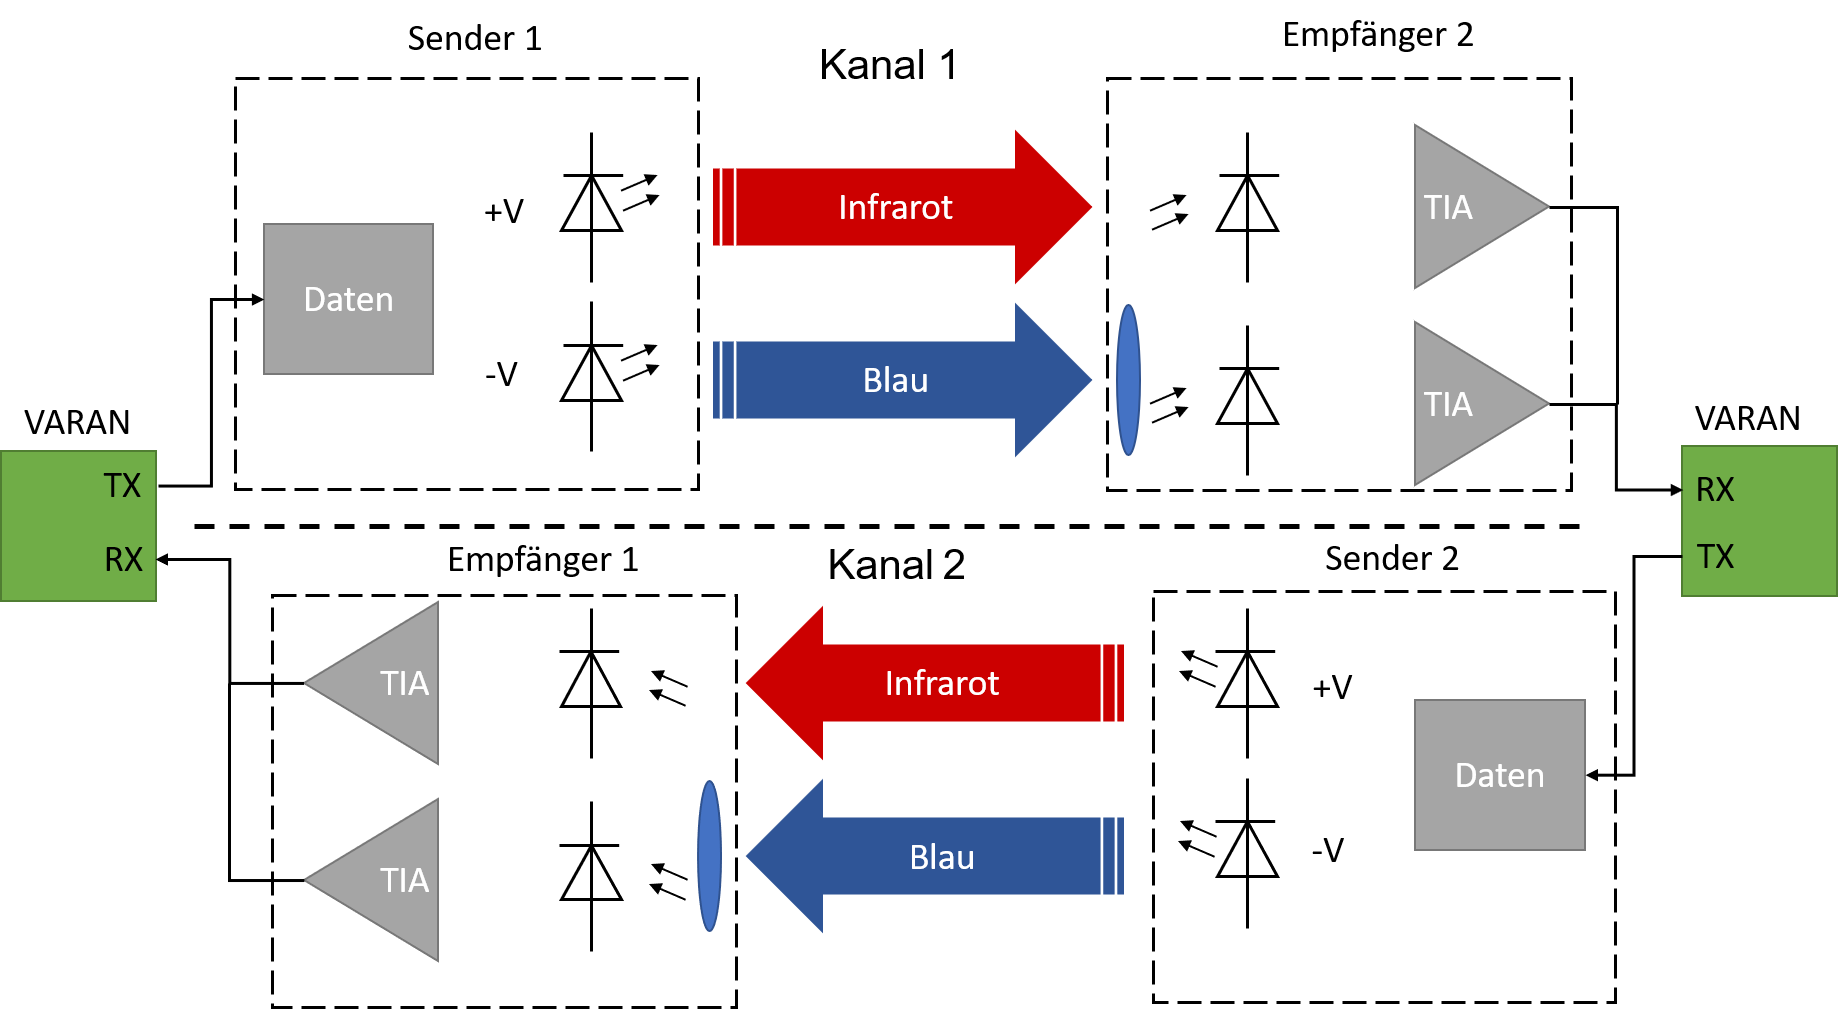
\includegraphics[width=\linewidth]{Konzept_Daten.png}
	\caption{Konzept der optischen Datenübertragung}\label{fig:Konzept_Daten}
\end{figure}

In Abbildung \ref{fig:Konzept_Daten} sind die beiden Kanäle zu erkennen, welche optisch voneinander getrennt sind. Jeder Kanal überträgt dabei die Daten nur in jeweils eine Richtung. Beide Kanäle zusammen sorgen für die gewünschte Bidirektionalität. Auf der Primär- und Sekundärseite hat es jeweils eine Sende- und Empfangseinheit. Eine Sendeeinheit besteht aus der Datenerfassung und den Leuchtdioden. 
\newline
Da der VARAN-Bus MLT-3 codiert ist, müssen drei Zustände übertragen werden können. Die positiven Spannungspegel werden mit einer Infrarot-LED übertragen und die negativen Spannungspegel mit einer blauen LED. Der Zustand \glqq0\grqq steht an, wenn keine der LEDs leuchtet.
\newline
Eine Empfangseinheit besteht aus Photodioden, Verstärkerschaltungen und der Pegelanpassung. Im blauen Spektralbereich werden mit Hilfe eines optischen Filters vor der Photodiode die unerwünschten Spektralanteile herausgefiltert.
\newline Die beiden Sende- und Empfangseinheiten sind identisch aufgebaut und unterscheiden sich nur in der Übertragungsrichtung.

\paragraph{Sender}
In folgender Abbildung ist das Konzept einer Sendeeinheit detaillierter dargestellt.

\begin{figure}[H]
	\centering
	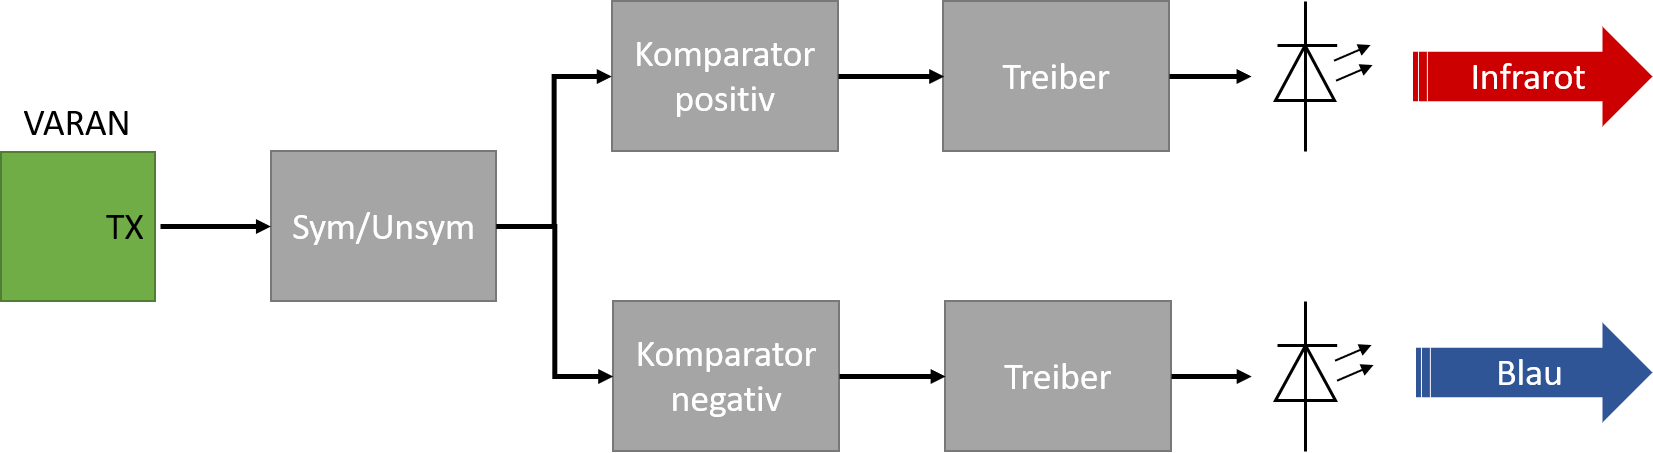
\includegraphics[width=\linewidth]{Konzept_Sender.png}
	\caption{Konzept der optischen Sendeeinheit}\label{fig:Konzept_Sender}
\end{figure}

Aus dem symmetrischen Signal des VARAN-Buses wird zuerst ein asymmetrisches Signal erzeugt. Dafür wird ein Signal-Transformator eingesetzt. Das Signal erhält so einen Bezug zur Masse der restlichen Schaltung. Mit zwei Komparatoren wird unterschieden, ob es sich um einen positiven oder negativen Pegel handelt. Dafür werden Komparatoren mit möglichst kurzer Verzögerungszeit und ausreichender Bandbreite verwendet. Die Komparatoren steuern anschliessend die entsprechenden Treiber an. 
\newline
Als Treiber dient ein FET-Treiber Baustein mit hoher Treiberspannung für schnelle Anstiegs- und Abfallzeiten. Die LED wird mit einem N-Kanal-FET nach Masse geschaltet. Die Schaltzeiten der LED sind entscheidend um auf die geforderte Schaltfrequenz von \textgreater \SI{30}{MHz} zu kommen. Dafür wurde einerseits ein FET mit kleiner Gate-Kapazität gewählt und andererseits auf kurze Anstiegs- und Abfallzeiten der LED geachtet.
\newline
Mit einer Erweiterung der Beschaltung der LED um drei passive Elemente, können die Anstiegs- und Abfallzeiten bei Bedarf um mehr als 50\% reduziert werden. Abbildung \ref{fig:Fast_LED} zeigt die Ansteuerung der LED mitsamt der Erweiterung von $R_{2}$, $C$ und $L$.

 \begin{figure}[h]
 	\centering
 	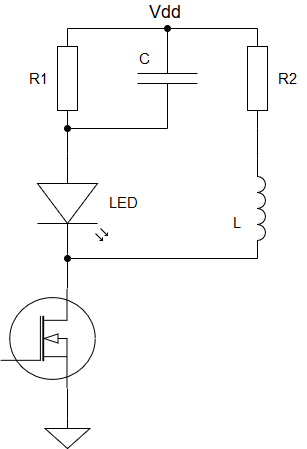
\includegraphics[width=0.3\linewidth]{Fast_LED.png}
 	\caption{Erweiterte Schaltung um Schaltzeiten zu verkürzen}\label{fig:Fast_LED}
 \end{figure}

Durch den Leckstrom des FET wird die LED auch im abgeschalteten Zustand mit einigen Ladungsträgern durchflossen, was die Anstiegszeit geringfügig verkürzt. Im Einschaltmoment sorgt der Kondensator $C$ für einen Kurzschluss und überbrückt den Vorwiderstand $R_{1}$. Es kommt zu einem Strompeak, der die Kapazität der LED schneller laden lässt. Die Anstiegszeit wird dadurch massiv verkürzt. Im Ausschaltmoment induziert das Magnetfeld in der Spule $L$ eine negative Spannung. Folglich werden die Ladungsträger aus der LED gezogen. Dadurch wird auch die Abfallzeit gegenüber dem \glqq einfachen\grqq Ausschalten verkürzt.\textcolor{red}{[paper]}

\paragraph{Empfänger}
In folgender Abbildung wird das Konzept einer Empfangseinheit detaillierter dargestellt.

\begin{figure}[h]
	\centering
	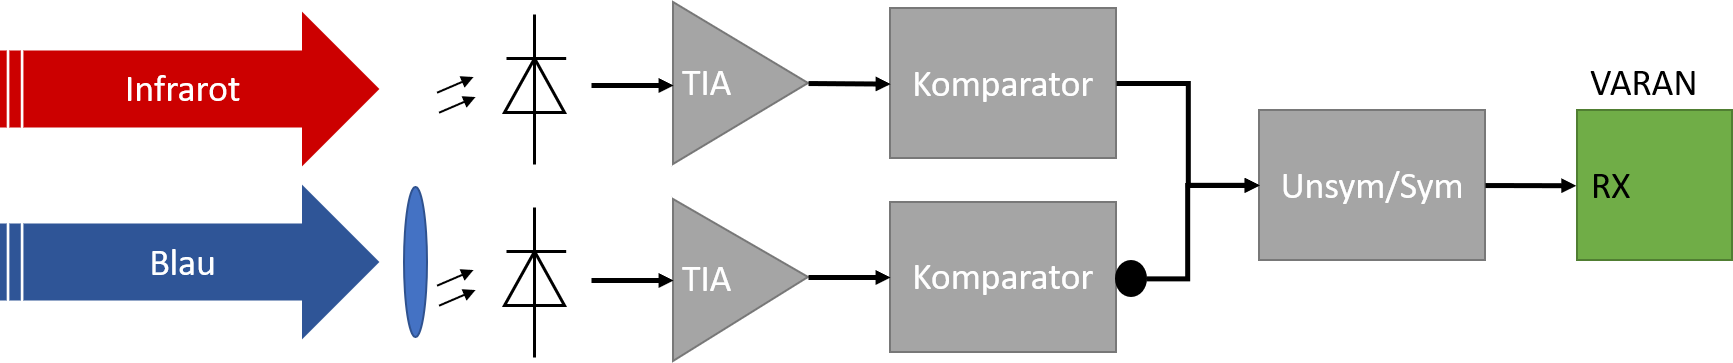
\includegraphics[width=\linewidth]{Konzept_Empfaenger.png}
	\caption{Konzept der optischen Empfangseinheit}\label{fig:Konzept_Empfaenger}
\end{figure}

Der von der Photodiode erzeugte Strom wird mit einer Transimpedanzverstärkerschaltung in eine Spannung gewandelt und verstärkt. Wie im Kapitel \nameref{sec:Grundlagen} bereits erwähnt, ist eine hohe Bandbreite bei der Verstärkerschaltung erforderlich. Deshalb ist ein Verstärker mit hohem Gain-Bandwidth Product und kleiner Eingangskapazität zu wählen. Auch die parasitäre Kapazität der Photodiode beeinflusst die Bandbreite, weshalb auch diese möglichst klein gewählt werden muss. Durch negative Biasspannung an der Anode kann die Kapazität nochmals reduziert werden.
\newline
Nach dem Transimpedanzverstärker werden mit Komparatoren die Pegel in Amplitude und Form angepasst. Das Signal vom blauen Spektralbereich, welches die negativen Pegel überträgt wird noch invertiert. Mit einem Signal-Transformator wird aus dem unsymmetrischen Signal wieder ein symmetrisches Signal generiert und dieses zurück an den VARAN-Bus geführt.

\paragraph{Kanal}
Da die optische Übertragung auf einer drehbaren Konstruktion stattfindet, ist keine direkte Verbindung sichergestellt. Deshalb bestehen die beiden Kanäle aus einem lichtstreuenden Werkstoff und sind optisch voneinander isoliert. Nachfolgende Abbildung zeigt den prinzipiellen Aufbau der Kanäle.

\begin{figure}[h]
	\centering
	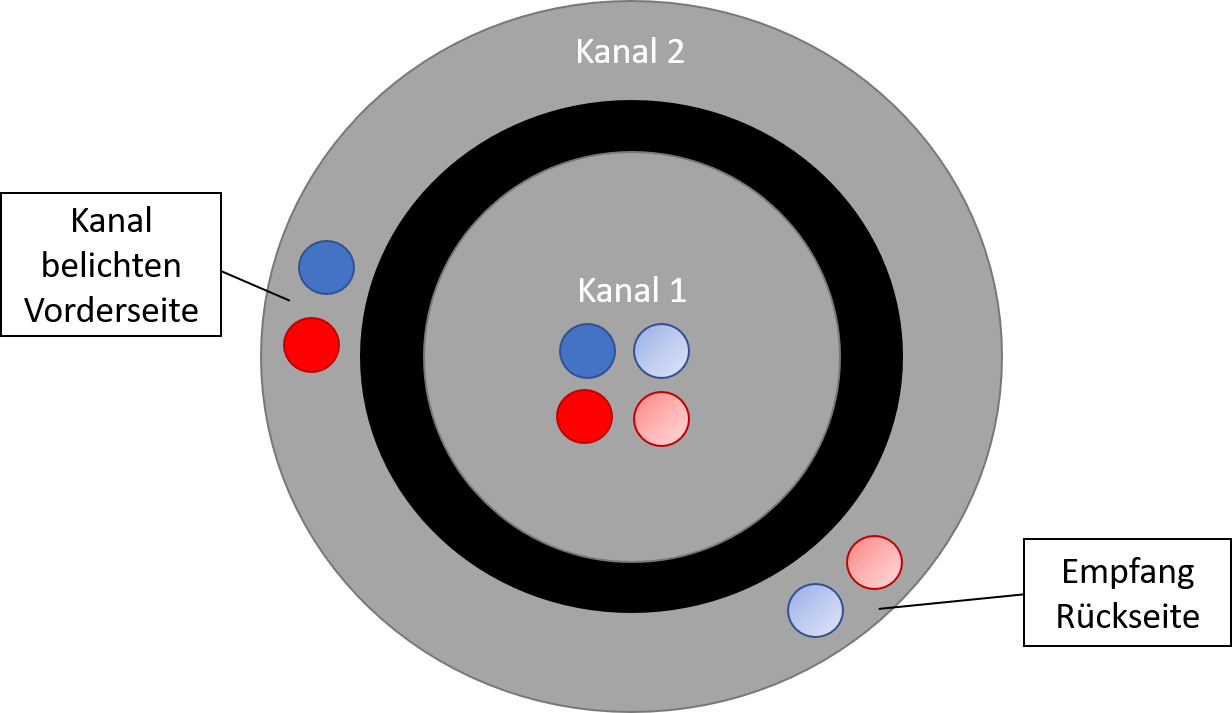
\includegraphics[width=0.6\linewidth]{Konzept_Kanal.png}
	\caption{Konzept der Kanäle}\label{fig:Konzept_Kanal}
\end{figure}

In der Abbildung ist die optische Isolation (schwarz) gut zu erkennen, welche die gegenseitige Beeinflussung der beiden Kanäle verhindert. Im Kanal 1 ist die Rotation der mechanischen Konstruktion unproblematisch, da sich Sender und Empfänger auf der Drehachse befinden. Der Kanal 2 nimmt das Licht auf der einen Seite auf und der lichtstreuende Werkstoff (grau) verteilt es im ganzen Kreisring. Nun spielt es auf der Empfängerseite keine Rolle mehr, in welchem Abschnitt auf dem Kreisring man sich befindet.

\subsection{Dimensionierung Testaufbau}
Es wurde ein Testaufbau realisiert, um für den weiteren Projektverlauf folgende Erkenntnisse zu gewinnen:
\begin{itemize}
	\item Kann die geforderte Geschwindigkeit erreicht werden?
	\item Welche Distanz ist möglich?
	\item Empfindlichkeit auf Umgebungslicht 
\end{itemize}
Der Testaufbau beinhaltet eine Sende- und Empfangseinheit, um ein Rechtecksignal im Infrarotbereich zu übertragen. 
In diesem Unterkapitel wird auf die wichtigsten Punkte zur Dimensionierung des Testaufbaus eingegangen. Das entsprechende Schema mit der Detailbeschaltung ist dem Anhang zu entnehmen.
\paragraph{Sender} 
Als Eingang beim Sender dient eine BNC-Buchse, um das Rechtecksignal einzuspeisen. Als Gatetreiber des FET wird der ISL55110 vom Hersteller Renesas verwendet. Dieser zeichnet sich durch kurze Anstiegs- und Fallzeiten von \SI{1.5}{ns} bei einer Last von \SI{100}{pF} aus.
Der gewählte N-Kanal-FET ist ein BSS316N vom Hersteller Infineon. Durch die kleine Eingangskapazität von \textless \SI{100}{pF} kann der FET in Kombination mit dem Gatetreiber sehr schnell geschaltet werden.
Als Infrarot-Emitter wurde die SFH4235 von OSRAM gewählt. Die Leuchtdiode kann mit Anstiegs- und Abfallzeiten von 7/\SI{14}{ns} mit \textgreater \SI{30}{MHz} betrieben werden und ist deshalb für diese Anwendung geeignet. Folgende Abbildung zeigt das Spektrum des Infrarot-Emitters.

\begin{figure}[h]
	\centering
	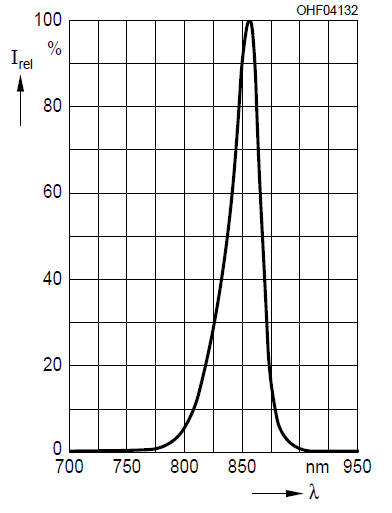
\includegraphics[width=0.4\linewidth]{Spektrum_Infra.png}
	\caption{Spektrum SFH4235}\label{fig:Spektrum_Infra}
\end{figure}

Wie in der Abbildung zu erkennen ist, hat das Spektrum den Peak bei \SI{860}{nm}. Die Photodiode auf der Empfängerseite muss dementsprechend passend zum Spektrum ausgewählt werden. Die im Konzept beschriebene Schaltungsergänzung wurde im Testaufbau vorbereitet. Weil die einfache Ansteuerung schnell genug ist, wird die Ergänzung vorerst nicht bestückt.

\paragraph{Empfänger}
Mit zwei Z-Dioden (SZBZX84C3V3 und BZD27C13) und einem Operationsverstärker (LM7321) als Buffer geschaltet, wird eine Speisung für die Empfängerschaltung generiert. Diese liefert die benötigten Spannungen von \SI{3.3}{V} für die integrierten Bauteile und \SI{-13}{V} um die Photodiode mit einer negativen Biasspannung vorzuspannen. Die Beschaltung ist im Schema im Anhang abgebildet.
\newline
Es wurden drei verschiedene Photodioden ausgewählt und analysiert.

\begin{table}[H]
\begin{tabular}{|l|l|l|l|}
	\hline 
	\textbf{Typ}&\textbf{$C_{p} (V_{R}=\SI{0}{V})$}  & \textbf{$C_{p} (V_{R}=\SI{-13}{V})$} & \textbf{Wellenlänge max. Sensitivität} \\ 
	\hline 
	SFH 203 FA Osram&\SI{11}{pF}  & \SI{2.5}{pF} & \SI{900}{nm} \\ 
	\hline 
	SFH 2701 Osram&\SI{3}{pF}  &\SI{1.7}{pF}  &\SI{820}{nm}  \\ 
	\hline 
	S5972 Hamamatsu&\SI{6}{pF}  &\SI{2.8}{pF}  &\SI{800}{nm}  \\ 
	\hline 
\end{tabular} 
\caption{Datenblattwerte der ausgewählten Photodioden}\label{tab:Tabelle_Photo}
\end{table}

Wie aus der Tabelle zu entnehmen ist, kann die parasitäre Kapazität aller ausgewählten Photodioden durch die negative Biasspannung auf einen Wert \textless \SI{3}{pF} gebracht werden. Dieser Wert dient als Ausgangslage für weitere Berechnungen und Simulationen.
\newline
Um einen Anhaltspunkt für den zu erwartenden Photostrom zu haben, wurden die Photodioden bei Bestrahlung mit dem Infrarot-Emitter ($I_{F}=\SI{280}{mA}$, konstant) ausgemessen.

\begin{figure}[h]
\centering
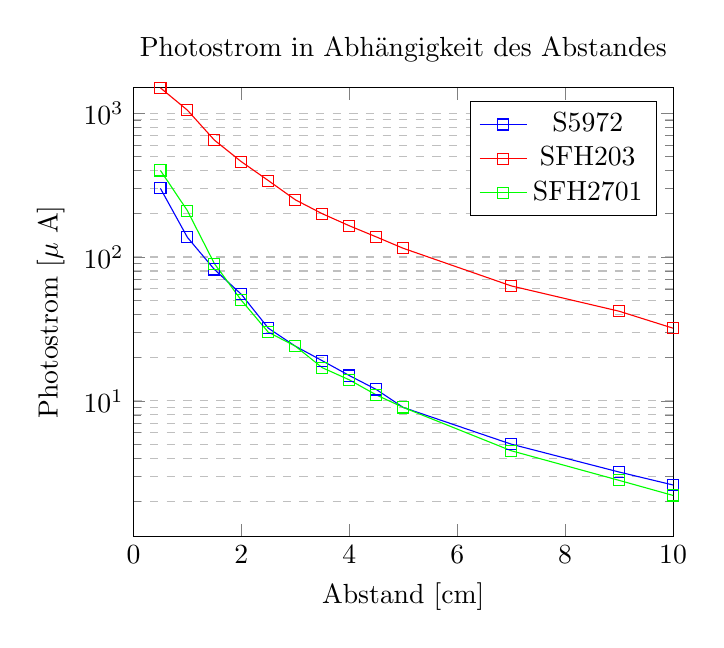
\begin{tikzpicture}
\begin{axis}[
title={Photostrom in Abhängigkeit des Abstandes},
xlabel={Abstand [cm]},
ylabel={Photostrom [$\mu$ A]},
xmin=0, xmax=10,
ymin=0, ymax=1500,
ymode=log,
xtick={0,2,4,6,8,10},
%ytick={0,5,10,50,100,500,1000},
legend pos=north east,
ymajorgrids=true,
yminorgrids=true,
grid style=dashed,
]

\addplot[
color=blue,
mark=square,
]
coordinates {
	(0.5,300)(1,137)(1.5,82)(2,55)(2.5,32)(3,24)(3.5,19)(4,15)(4.5,12)(5,9)(7,5)(9,3.2)(10,2.6)
};

\addplot[
color=red,
mark=square,
]
coordinates {
	(0.5,1500)(1,1050)(1.5,650)(2,460)(2.5,340)(3,250)(3.5,200)(4,165)(4.5,138)(5,115)(7,63)(9,42)(10,32)
};

\addplot[
color=green,
mark=square,
]
coordinates {
	(0.5,400)(1,210)(1.5,90)(2,50)(2.5,30)(3,24)(3.5,17)(4,14)(4.5,11)(5,9)(7,4.5)(9,2.8)(10,2.2)
};
\legend{S5972,SFH203,SFH2701}

\end{axis}
\end{tikzpicture}
\caption{Photostrom in Funktion des Abstands verschiedener Photodioden}\label{fig:Plot_Photo}
\end{figure}

Aus der Grafik geht hervor, dass bei einer Distanz von \SI{4}{cm} mit einem Photostrom von \textgreater $\SI{10}{\mu A}$ gerechnet werden kann. Diese Distanz wurde abgeschätzt und hängt von der späteren mechanischen Konstruktion ab. Sie dürfte aber eher kleiner werden, weshalb diese Annahme getroffen wurde.
\newline
Als Transimpedanzverstärker wurde der LT6268 von Linear Technology gewählt. Dieser Verstärker ist durch sein hohes GBWP von \SI{4}{GHz} und der kleinen Eingangskapazität von \SI{0.45}{pF} für High-Speed Photoanwendungen geeignet.

Gemäss Formel \ref{eq:Bandwidth} ist mit diesem Verstärker in Kombination mit einer der ausgewählten Photodioden folgende Bandbreite möglich:

\begin{equation}\label{eq:Bandwidth2}
B=\sqrt{\frac{GBWP}{2\pi\cdot R_{f}\cdot (C_{opamp}+C_{photo})}}\approx \SI{96}{MHZ}
\end{equation}

Dabei wurde mit $R_{f}=\SI{20}{k\Omega}$, $GBWP=\SI{4}{GHz}$, $C_{opamp}=\SI{0.45}{pF}$ und $C_{photo}=\SI{3}{pF}$ gerechnet.

Gemäss Datenblatt des Verstärkers braucht es eine Kapazität im Feedback-Loop für eine stabile Funktionalität im höheren Frequenzbereich. Dafür gelten folgende Bedingungen:
\begin{equation}\label{eq:Amp_Cf}
C{f}\textgreater \sqrt{\frac{C_{IN}}{\pi\cdot GBWP\cdot R_{f}}}
\end{equation}

\begin{equation}\label{eq:Cin_Cf}
\frac{C_{IN}}{C_{f}}\geq 10
\end{equation}

Mit den beiden Formeln \ref{eq:Amp_Cf} und \ref{eq:Cin_Cf} bekommt man folgende Bedingung für $C_{f}$: 
\begin{equation}\label{eq:Cfminmax}
\SI{150}{fF}\textgreater C_{f}\textgreater \SI{500}{fF}
\end{equation}

Aufgrund der Dimensionierung der Sende- und Empfangsschaltung, wird in LTSpice ein Simulationsmodel erstellt.
\todo[inline]{ Unterkapitel noch abschliessen und zur Simulation überleiten}

\subsection{Simulation}
Die im vorherigen Kapitel durchgeführte Dimensionierung soll nun anhand einer Simulation überprüft werden.
Dafür wurde die Empfängerschaltung gemäss Schema im Anhang in LTSpice gezeichnet. Abbildung \ref{fig:PhotoAmp_Concept} zeigt die Prinzipschaltung. Die genaue Simulationsschaltung befindet sich im Anhang.
\begin{figure}[h]
	\centering
	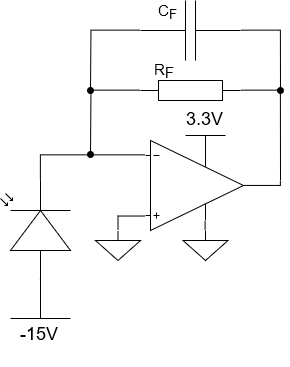
\includegraphics[width=0.3\linewidth]{PhotoAmp_Concept.png}
	\caption{Empfängerschaltung}\label{fig:PhotoAmp_Concept}
\end{figure}

Um den Einfluss der Kapazität in der Rückkopplung $C_{f}$ gemäss Bedingung \ref{eq:Cfminmax} zu überprüfen, wurde ein Parameter-Sweep mit mehreren Werten durchgeführt. Es wurden folgende Kapazitäten simuliert: \SI{50}{fF}, \SI{100}{fF}, \SI{200}{fF}, \SI{300}{fF}, \SI{400}{fF} und \SI{500}{fF}. Als Photostrom wurden Reckteck-Pulse mit einer Amplitude von \SI{10}{\mu A} gemäss Dimensionierung gewählt und einer Wiederholungsfrequenz von \SI{33}{MHz}.
Abbildung \ref{fig:Plot_Cf} zeigt das Ausgangssignal des Transimpedanzverstärkers bei verschiedenen Feedback-Kapazitäten zusammen mit dem Eingangsstrom.
\begin{figure}[H]
	\centering
	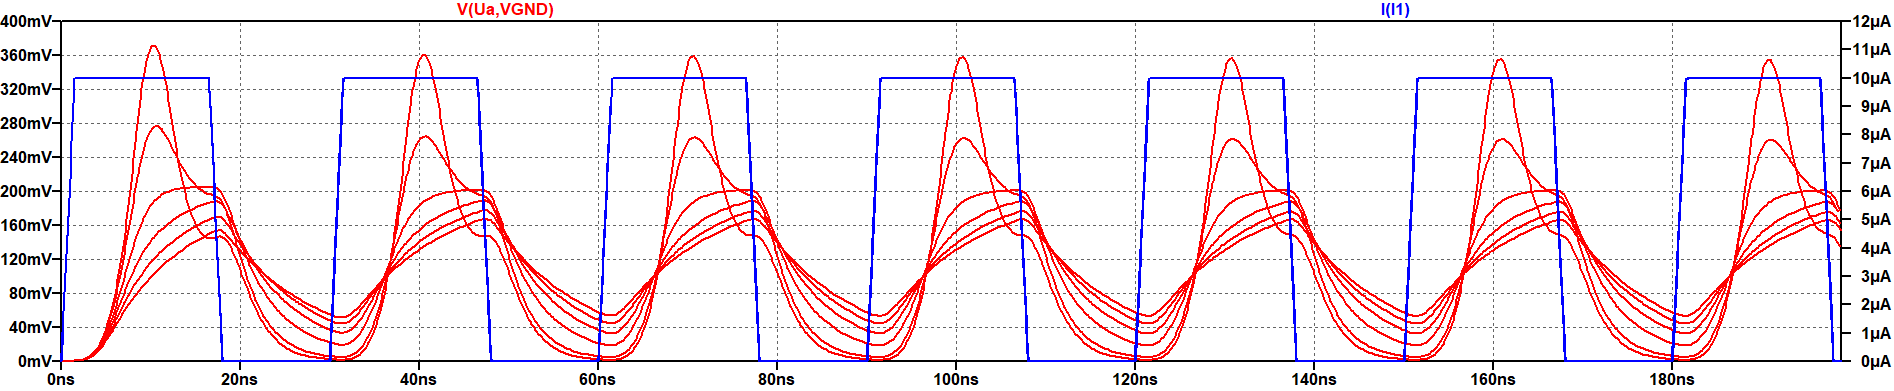
\includegraphics[width=\linewidth]{LTPlot_Cf.png}
	\caption{Eingangsstrom und Ausgangsspannung bei verschiedenen Feedback-Kapazitäten}\label{fig:Plot_Cf}
\end{figure}
In der Abbildung \ref{fig:Plot_Cf} sind bei kleinen Kapazitätswerten hohe Überschwinger zu erkennen. Bei grösseren Kapazitäten ändert die Spannung zu langsam. Von den simulierten Werten liefert eine Kapazität von \SI{200}{fF} das beste Resultat. Abbildung \ref{fig:Plot_Cf200} zeigt die \SI{200}{fF}-Kurve alleine.

\begin{figure}[H]
	\centering
	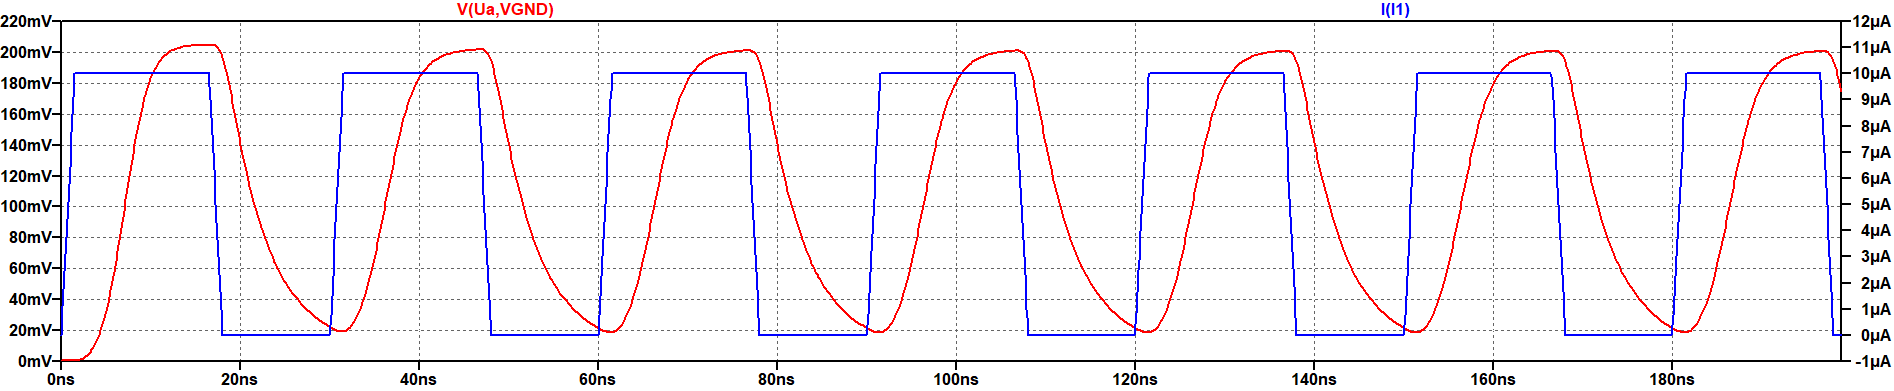
\includegraphics[width=\linewidth]{LTPlot_Cf200.png}
	\caption{Eingangsstrom und Ausgangsspannung bei $\SI{200}{fF}$ Feedback-Kapazität}\label{fig:Plot_Cf200}
\end{figure}

Mit einem Komparator kann nun aus dem Signal wieder das gewünschte Rechtecksignal erzeugt werden. Abbildung \ref{fig:Plot_out} zeigt das Ausgangssignal nach der Pegelanpassung durch den Komparator LTC6752.

\begin{figure}[H]
	\centering
	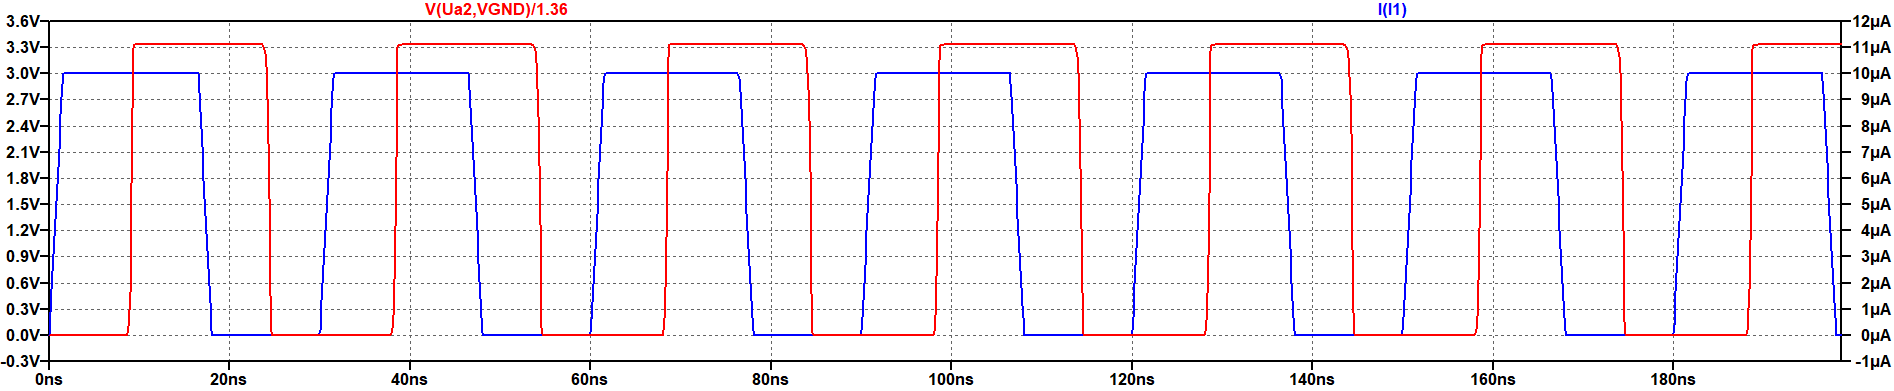
\includegraphics[width=\linewidth]{LTPlot_out.png}
	\caption{Eingangsstrom und Ausgangsspannung bei $\SI{200}{fF}$ Feedback-Kapazität mit Komparator}\label{fig:Plot_out}
\end{figure}




\subsection{Testaufbau}
\label{subsec:Testaufbau}
Um die entwickelten Sende- und Empfangsschaltung auszumessen, wurde ein Testaufbau erstellt.

Dafür wurde eine \SI{8}{mm} dicke Acryl-Satlite-Platte vom Hersteller \glqq BWF-Profiles\grqq\  in eine \SI{6x6}{cm} Scheibe zugeschnitten. Anschliessend wurde das Licht-Signal

\subsection{Validierung} 

Für die Validierung der Sende- und Empfangsschaltung wurden Messungen gemäss Beschreibung im Unterkapitel \nameref{subsec:Testaufbau} durchgeführt. Damit soll die geforderte Geschwindigkeit und der Einfluss von Störlicht überprüft werden. Zusätzlich wird eine Messung durch eine Acryl-Scheibe durchgeführt, welches später als lichtleitendes Material für den Kanal dienen soll.
 
\paragraph{Geschwindigkeit}
Wie in den \nameref{sec:Grundlagen} mit Formel \ref{eq:MLT3} gezeigt, soll eine Frequenz von \SI{31.25}{MHz} erreicht werden. Messungen bei direktem Sichtkontakt zwischen Infrarot-Emitter und Photodiode auf eine Entfernung von ca. \SI{4}{cm} ergaben die in Abbildung \ref{fig:output33_40} gezeigten Resultate.

\begin{figure}[h!]
	\centering
	\subfloat[\SI{33}{MHz}]{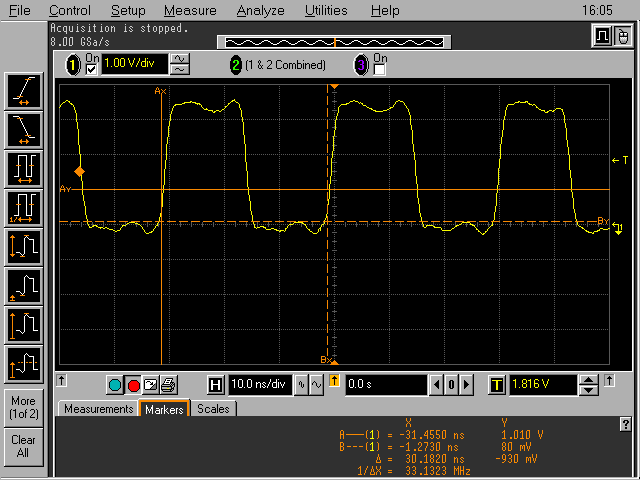
\includegraphics[width=0.47\linewidth]{output33MHz.png}}\qquad
	\subfloat[\SI{40}{MHz}]{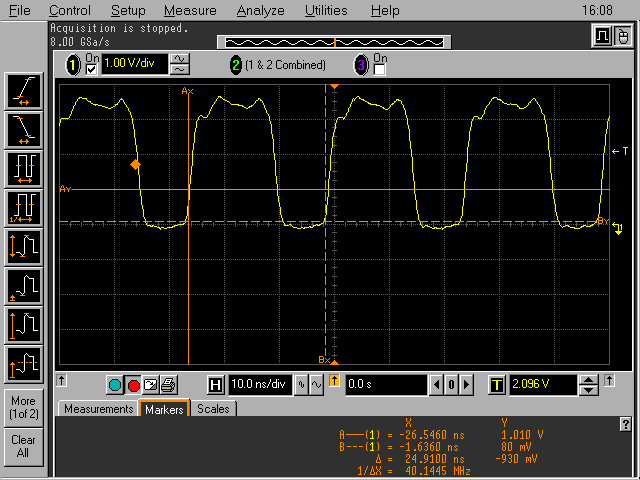
\includegraphics[width=0.47\linewidth]{output40MHz.png}}
	\caption{Ausgangssignal der Empfängerschaltung bei direktem Sichtkontakt über \SI{4}{cm}}
	\label{fig:output33_40}
\end{figure}

Sowohl \SI{33}{MHz} als auch \SI{40}{MHz} können mit diesem Testaufbau übertragen werden. Abbildung \ref{fig:output45} zeigt die maximal erreichte Frequenz in dieser Konfiguration.


\begin{figure}[h!]
	\centering
	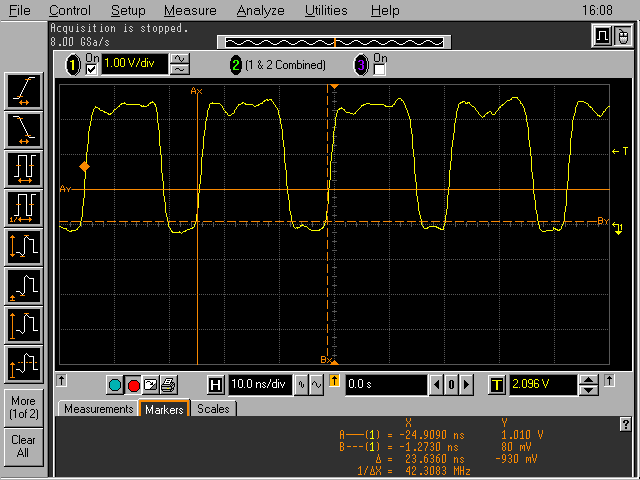
\includegraphics[width=0.7\linewidth]{output45MHz.png}
	\caption{Ausgangssignal der Empfängerschaltung bei \SI{45}{MHz}}
	\label{fig:output45}
\end{figure}

Mit den gemessenen \SI{45}{MHz} ist die geforderte Frequenz von \SI{31.25}{MHz} deutlich erreicht. Die benötigte Geschwindigkeit für eine berührungslose Übertragung des VARAN-Bus kann mit dieser Schaltung erreicht werden.

\newpage
\paragraph{Übertragung durch Kanal}
Als weitere Messung wird die Übertragung durch eine Acryl-Scheibe durchgeführt. In Abbildung \ref{fig:plexi33} wird das Empfangene Signal am Ausgang der Empfängerschaltung gezeigt.
\begin{figure}[h!]
	\centering
	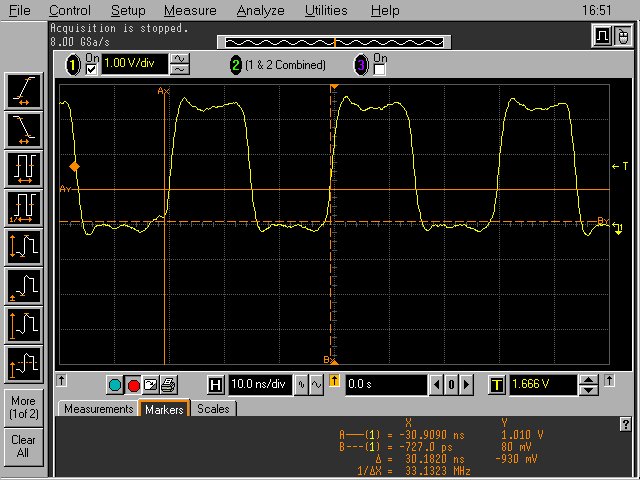
\includegraphics[width=0.7\linewidth]{plexi33MHz.png}
	\caption{Ausgangssignal der Empfängerschaltung bei \SI{33}{MHz} durch Acryl-Scheibe}\label{fig:plexi33}
\end{figure}
Das Licht wird im Acrylglas gebündelt und durch das Material geleitet. Bei der Vergleichsmessung ohne Acryl-Platte war der Signalpegel am gleichen Empfangspunkt hingegen zu schwach, um den Komparator zu schalten. Auch wenn an der Kante eingespeist wird und auf der Oberfläche gemessen wird, ist der Pegel zu schwach. Acrylglas ist als lichtleitendes Material eine geeignete Wahl. Mit Anpassungen am Verstärkungsfaktor des Transimpedanzverstärkers und der Schaltschwelle für den Komparator wären noch bessere Resultate möglich. Durch Rücksprache mit dem Hersteller dürfte noch ein besseres Material gefunden werden, um mit einer geschickten Konstruktion den konzipierten Kanal herzustellen.

\paragraph{Störlicht}
Sämtliche Messungen wurden bei Tageslicht und Sonneneinstrahlung durchgeführt. Dabei wurden keine Unregelmässigkeiten registriert, welche vom Umgebungslicht stammen könnten. Da der Dosenverschliesser in einem Gebäude eingesetzt wird und durch die Konstruktion kaum Licht in die Schaltung eindringen wird, kann die Schaltung als störsicher gegen Umgebungslicht eingestuft werden.